\documentclass{article}
%\usepackage[utf8]{inputenc}
\usepackage{hyperref}
\usepackage{graphicx}
\usepackage{float}
%\usepackage{listings}

\title{Assignement 5}
\author{Iván Piña Arévalo \\ ivan.pinaarevalo@alum.uca.es}
\date{\today}

\begin{document}
\maketitle

\newpage
\begin{abstract}
    En esta práctica realizaremos una aproximación del Travelling Salesman Problem (TSP). Este problema es bien conocido 
    NP-Hard, por lo que encontrar la solución óptima es tiempo polinomial no es posible a día de hoy.  Para la aproximación hemos 
    empleado un enfoque genético. Usamos dos operadores de cruce distintos, analizando el resultado de cada uno. Así mismo 
    dotamos al programa de un factor de aleatoriedad importante de cara a aumentar la anchura del espacio de estados explorado. 
\end{abstract}

\newpage
\section{Introduction}
    Comenzaremos hablando del Travelling Salesman Problem. Consiste en dada una serie de ciudades, encontrar la secuencia de ciudades tal que la distancia de recorrerlas 
    sea mínima, partiendo de un origen y finalizando en él. Como se puede observar conforme se aumenta el número de ciudades, ocurre
    una explosión del número de posibles combinaciones. Por esto un enfoque de fuerza bruta no es precisamente apropiado. En lugar 
    de encontrar la solución óptima, podemos emplear algoritmos computables que den una aproximación de la solución óptima, es decir, 
    no la mejor solución pero si una lo suficientemente aceptable. 

    Podemos utilizar dos tipos de algoritmos para realizar la aproximación:
    \begin{itemize}
        \item Ant Colony Optimisation: Basado en el mecanismo que emplean las hormigas para encontrar la ruta mas corta 
        entre su colonia y posibles comidas. A grandes rasgos podríamos decir que cada hormiga trabajadora va dejando feromonas 
        a su paso. Consecuentemente el camino más corto poseerá mas feromonas que el resto de caminos (al poder realizar en menos 
        tiempo la ruta). Las demás hormigas a su vez toman el camino que mas feromonas posee (se induce que es más corto, más seguro, etc.).
        De esta forma la colonia de hormigas determina cuál es el camino más corto. 
        \item Genetic Algorithm: Esta basado en la teoría de la evolución. Parte de una población inicial de individuos y a través 
        de cruces, mutaciones y reemplazos la población se va quedando con los individuos mejor adaptados (es decir, aquellos que 
        dada una función de evaluación saquen una mayor puntuación.)
    \end{itemize}

    He decidido emplear Algoritmos Genéticos para la aproximación. Aunque a simple vista la colonia de hormigas es más 
    intuitivo, opino que los algoritmos genéticos poseen más mecanismos para adaptar el esquema básico de un algoritmo genético 
    al Travelling Salesman Problem. No obstante también es verdad que el rendimiento de un algoritmo genético se ve seriamente 
    afectado por la configuración de sus paramétros. Consecuencia de esto se podría realizar un estudio que únicamente trate acerca
    de la configuración de los paramétros. 
    
\section{Methodology}
A continuación pasamos a detallar cada una de las partes que componen el algoritmo. Como se podrá observar conforme avance la
lectura, existen varias partes que son generadas de manera aleatoria (es decir, sin un orden definido). En dichas partes se ha 
hecho uso de la funcion $rand()$ definida en $<stdlib.h>$

Para llamar la programa debemos pasarle como argumento el nombre del fichero que contiene el mapa. Un ejemplo de llamada es:
\\ 
\hspace{5mm} ./a.out $./Maps/eil51.tsp$ 

\subsection{Mapas seleccionados}
    Dado que para el análisis es suficiente con evaluar 5 mapas, hemos elegido mapas en los que las coordenadas de cada ciudad 
    sean números enteros. Hemos utilizado los siguientes mapas:
    \begin{itemize}
        \item eil51.tsp
        \item eil76.tsp
        \item kroaA100.tsp
        \item eil101.tsp
        \item a280.tsp
    \end{itemize}

\subsection{Gen}
    En primer lugar debemos definir lo que van a ser los individuos de la población, llamados genes. Cada gen es una estructura 
    que posee dos campos:
    \begin{itemize}
        \item vector con las ciudades: Define el orden en que se recorren las ciudades. 
        \item coste: Almacena la distancia que implicar recorrer las funciones en el orden que contiene el vector, partiendo de 
        la primera posición y volviendo finalmente a ella desde la última posición del vector. 
    \end{itemize} 

\subsection{Poblacion}
    Esta formada por un conjunto de genes. Para generarla, he diseñado dos funciones:
    \begin{itemize}
        %sugiero cambiar nombre a generar_gen
        \item generar\_elemento: Genera una secuencia aleatoria con todas las ciudades. Es importante que la secuencia sea 
        aleatoria para explorar la mayor parte posible del espacio de estados. 
        \item generar\_poblacion: Se apoya en la función generar\_elemento para ir creando los genes que formarán la población. 
    \end{itemize}

\subsection{Función de evaluación}
    Hemos empleado la distancia eúclidea. La distancia eúclidea se define como: 
        \[d(P_1,P_2)= \sqrt{ (x_2 - x_1)^2 +(y_2-y_1)^2} \]
    Consecuentemente, el coste o puntuación asignado a un candidato será la suma de las 
    distancias entre una ciudad y su siguiente, mas desde la última ciudad a la primera.  

\subsection{Best solution}
    Es la mejor puntuación obtenida de toda la población. En base a la diferencia de este paramétro con la solución óptima 
    podemos estimar el rendimiento del algoritmo. Así mismo también se puede utilizar como condición de parada si esta es 
    lo suficientemente buena o si las variaciones de su valor en las últimas iteraciones no es lo suficientemente grande. 
    
\subsection{Selección de padres}
    Para seleccionar los padres empleo el método conocido como 'Ruleta'. Utilizo este método por varios motivos 
    \begin{itemize}
        \item Los individuos con una mejor puntuación tienen más posibilidades de ser elegidos. De esta manera inclinamos 
        la balanza hacia el elitismo. 
        \item Aunque los mejores individuos tiene más probabilidades de ser elegidos, sigue existiendo la opción de que sean 
        seleccionados padres con una peor valoración. 
    \end{itemize}  
    Cabe la posibildad de que genes con una mala puntuación generen un hijo con una buena puntuación. Recordando la frase 
    que me dijo mi profesor, Gabriel Guerrero Contreras: \\
        
    \hspace{5mm}"Padres feos pueden tener hijos guapos"
    
    De ahí el hincapié en buscar equilibrio entre elistismo y la posiblidad de que cualquiera sea elegido. 

\subsection{Algoritmos de cruce}
Hemos utilizado dos algoritmos de cruce distintos.
\subsubsection{Sequential Constructive Crossover (SCX)}
En este algoritmo buscamos generar un hijo con la secuencia más corta de ambos padres. Posee contadores para el padre y la madre 
y tiene en cuenta las ciudades que ya existen en el hijo a medida que lo va construyendo. El algoritmo se estructura en los 
siguientes pasos:
\begin{enumerate}
    \item Insertar la primera ciduad del padre. Incrementar el contador del padre para que apunte a su siguiente ciudad. 
    \item Buscar las ciudades del padre y de la madre. Puede ocurrir 4 escenarios posibles:
        \begin{itemize}
            \item Ni la ciudad del padre ni la de la madre están en el hijo: En este caso se busca la ciudad cuya distancia 
            a la última ciudad insertada en el hijo sea mayor. Se incrementa el contador del progenitor seleccionado. Aquí es donde 
            esta el elitismo en este operador. 
            \item La ciudad del padre no esta en el hijo pero la de la madre si: Se inserta la ciudad  del padre y se incrementan 
            ambos contadores (para saltar el ciudad de la madre que ya esta en el hijo.)
            \item La ciudad de la madre no esta en el hijo pero la del padre si: Se inserta el ciudad de la madre y se incrementan 
            ambos contadores (para saltar el ciudad del padre que ya esta en el hijo.)
            \item La ciudad del padre y la de la madre están ya en el hijo: En este caso lo único que hay que hacer es Incrementar
            los contadores de ambos.  Este caso aunque puede parecer raro es más común de lo que parece y ocurre cuando el elemento 
            al que apunta el padre ya ha sido insertado previamente por la madre y viceversa.%¿Este caso puede ocurrir realmente?
        \end{itemize}
    
    \item Repetir el paso nº2 hasta que todas las ciudades del mapa estén en el hijo. 
\end{enumerate}

\subsubsection{50\%}
En este algoritmo se divide al 50\% el primer progenitor y se inserta directamente en el hijo. A continuación insertamos 
las ciudades restantes del otro progenitor que no estén ya en el hijo. Además lo hacemos en el orden de aparición del otro 
progenitor, respetando en parte, ya que el orden se rompe debido a las ciudades que ya están en el hijo),el orden de las ciudades 
en el otro progenitor.  

\subsection{Mutación}
La función de mutación recibe dos paramétros a parte del candidato susceptible a ser mutado:
\begin{itemize}
    \item Probabilidad de mutación: Un valor entre 0 y 1. En dicha función se saca un valor aleatorio entre 0 y 1. Si dicho valor 
    es menor que la probabilidad de mutación, el gen será mutado. En caso contrario no ocurre la mutación. 
    \item Porcentaje de mutación: También es un valor entre 0 y 1. Dicho valor indica el porcentaje del gen que será mutado. 
\end{itemize}
    Para simular la mutación jugamos con el orden de las ciudades. Obtenemos dos posiciones aleatorias del array e intercambiamos 
    su valores. Así mismo el porcentaje del gen mutado no esta asegurado al 100\%. Esto es debido a que al obtener las posiciones 
    a intercambiar de manera aleatoria puede ocurrir que se elija mas de una vez la misma posición. 

\subsection{Reemplazamiento}
    Para el reemplazamiento hemos seguido también un enfoque aleatorio. Este enfoque presenta ventajas e inconvenientes 
    respecto a un enfoque elitista puro:
    \begin{itemize}
        \item Permite que genes con una menor puntuación sigan en la población: Como hemos mencionado antes, existe la 
        posibilidad de que genes con una baja puntuación generen hijos con buena puntuación. Esto lo considero una ventaja 
        respecto a un enfoque elitista porque expande más el espacio de estados.  
        \item Al mantener genes con una menor puntuación, la velocidad con la que se avanza hacia los mínimos detectados es 
        menor o puede que incluso no lleguen a alcanzarse dichos mínimos porque se pierdan los genes cuyos descendientes 
        llegasen a ese mínimo. 
    \end{itemize}    
\subsection{Condiciones de parada}
Empleamos dos condiciones de parada:
\begin{itemize}
    \item Variación en la mejor solución encontrada: Si la variación entre la mejor solución encontrada no varía un umbral
    respecto a la última iteracion, se considera que ha llegado a un mínimo y se finaliza la ejecución del algoritmo.
    \item Número máximo de iteraciones: Si el algoritmo no llega a estabilizarse tras un número suficiente de iteraciones, 
    finalizamos la ejecución del algoritmo. Con esta condición de parada evitamos caer en un bucle de duración indeterminada. 
\end{itemize}

\section{Results and Discussion}
%Aquí explica la configuración de los paramétros. 
Una posible configuración del algoritmo es esta:
\begin{itemize}
    \item Tamaño de la población: 1000 genes
    \item Número de hijos generados con cada población: 500 genes
    \item Probabilidad de mutación: 0.9
    \item Porcentaje de mutación: 0.8 
    \item Condición de parada: 200 iteraciones. También podriamos emplear que la variación entre el mejor elemento  respecto 
    a la anterior iteración sea $ < x$ y distinta de cero, pero para el análisis del algoritmo hemos empleado únicamente número 
    máximo de iteraciones. Si incluimos esta última condición necesitamos modificar x para cada mapa.   
\end{itemize}
Con esta configuración alcanzamos unos valores lejanos de cara a la solución óptima de los mapas. Tras modificar los paramétros y reflexionar 
sobre su comportamiento, el algoritmo se queda tan lejos de la solución principalmente por dos motivos:

\begin{itemize}
    \item Falta de un estudio previo acerca de los valores óptimos para cada paramétro: Es bien conocido que el resultado de los algoritmos 
    génetico esta fuertemente acoplado a los valores de sus paramétros. Como todos los paramétros influyen, es necesario un estudio previo acerca 
    de sus valores ideales.  
    \item Generalización de los paramétros: Hemos declarado los valores de los paramétros y a continuación hemos ejecutado el  algoritmo sobre 
    distintos mapas. Cada mapa posee un número distinto de ciudades, así como distinta posición cada ciudad. Por tanto la configuración de 
    paramétros debería realizarse para cada mapa de manera independiente. 
\end{itemize}


\subsubsection{SCX versus 50\%} 
Para que el tiempo de ejecución sea representativo, hemos puesto como condición de parada únicamente 
200 iteraciones. Hemos obtenido los siguientes resultados. 
%Utiliza un mapa para comparar ambos. 
\begin{figure}[H]
    \centering
    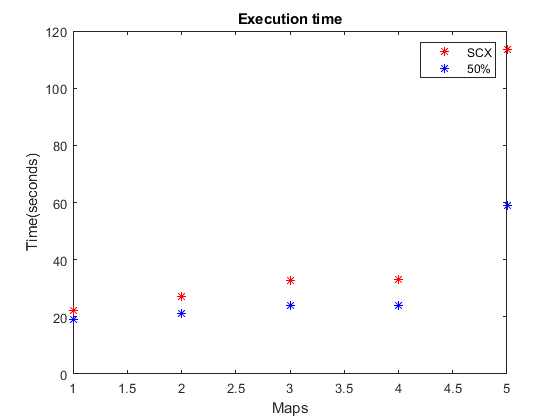
\includegraphics[width=1\textwidth]{tiempo.png}
    \caption{1-eil51 2-eil76 3-kroaA100 4-eil101 5-a280}
\end{figure}

Observarmos que el tiempo de ejecución es menor en el algoritmo 50\%. Asociamos estos resultados al hecho 
de que el algoritmo SCX es mas complejo. Tiene que buscar tanto en el padre como en la madre y si ambas 
ciudades se pueden insertar entonces calcula la ciudad mas cercana a la útima del hijo.  
Así mismo, si comparamos las puntuaciones obtenidas:

\begin{figure}[H]
    \centering
    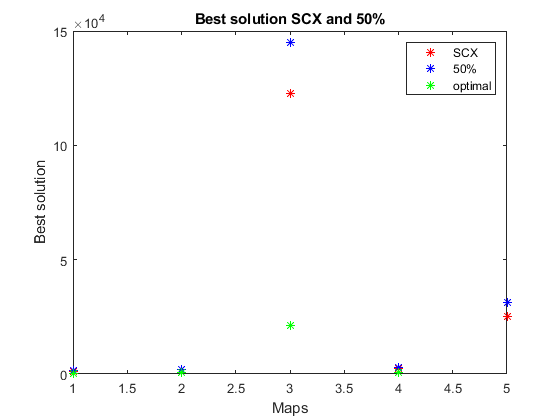
\includegraphics[width=1\textwidth]{solutions.png}
    \caption{1-eil51 2-eil76 3-kroaA100 4-eil101 5-a280}
\end{figure}
No disponemos de la solución óptima para el último mapa, por eso no aparece el asterisco verde en la 
posicion nº 5. 
Como se puede observar, el operador SCX obtiene mejores soluciones que el operador 50\%. Esto es debido 
a que SCX si tiene en cuenta la ciudad que es mas cercana respecto a la última ciudad insertada en 
el hijo (conforme se va creando el hijo.) En cambio el operador 50\% solo tiene en cuenta si puede añadir
la ciudad o no. 

\section{Conclussion}
    A nivel de operadores, observamos una relación tiempo-resultado. Si necesitamos encontrar 
    las mejores soluciones de estos dos algoritmos, interesa utilizar el operador SCX a cambio de sacrificar
    tiempo de computación. En cambio si utilizamos el operador 50\% sabemos que las soluciones serán 
    peores pero se consumirá menos tiempo de ejecución. 

    Como se puede observar, los resultados del algoritmo no son cercanos a la solución óptima. No obstante, calculamos en un tiempo razonable 
    una solución para un algoritmo NP-Hard. Bajo mi punto de vista es un gran avance ya que para muchos sistemas (GPS entre ellos) es ideal 
    pero no necesario encontrar la solución óptima.
    
    Así mismo, aunque no cambiaría el orden actual del algoritmo, se podría mejorar aún más el tiempo 
    de ejecución si paralelizasemos determinadas partes del algoritmo, por ejemplo la generación de parejas y la generación de hijos. Gracias 
    a las directivas de paralelización de C++ y el aumento en el número de núcleos del procesador, esta opción no es nada despreciable. 
    %... enfoque basto en aleatoriedad, lo que permite abarcar una mayor sección del espacio de estados. 
    %embargo como contrapartida no ahondamos avanzamos lo suficiente hacia los mínimos. 
\section{Bibliography}
\end{document}